
\tableofcontents
\chapter*{Introduction}

The goal of \tria software is to help the user to localize some problem roots in usual situation. Those situations have been described during a precedent step of the work. \tria software is aimed to give an easy acces to the most interesting informations.\\ 

%\tria est un logiciel permettant d'identifier facilement des lieux de problèmes dans des situations relationnelles courantes. Ces situations ont été schématisées au préalable et le but de \tria est de fournir un accès facile et rapide aux informations qui intéressent le plus l'utilisateur.\\

The second main function of \tria is to allow the user to transform most important schemes in personalized pictures. Then they could be used for a speech or in a report. As you can see in figure \ref{personalisation}, the user can apply a lot of enhancements.\\
%Dans un deuxième temps, \tria permet d'exporter les schémas importants sous la forme d'images afin de les utiliser dans le cadre d'une présentation ou d'un rapport. Il est possible de fortement personnaliser l'apparence des schémas lors de ces exportations pour les adapter au cadre d'utilisation.\\

The main steps of works with \tria are the followings : \\
%L'utilisation classique se déroule de la manière suivante :\\
\begin{enumerate}
\item Session creation, the user select the main actors for the situation he want to understand. It is possible to input the two telling for each actors.\\
\item Exploration of the different situations where the selected actors "do something". Each situation correspond to a brick. The "Global view" allow the user see all bricks with an automatic highlight of the probably most interesting bricks.\\
\item Input of real relations. Each brick contains some relation betweens the actors and the environment. The user have to input the real relation for each of them. Then the software highlight the relation which present a gap between the real situation and a correct theoric one.\\
\item Export of interesting informations. The user transforms the most interesting informations into pictures to explain the problems to the concerned persons.\\ 

%\item Création d'une session, l'utilisateur choisi dans une liste l'ensemble des acteurs concernés par la situation sur laquelle il veut travailler. Il est possible de saisir les deux récits des différents acteurs lors de cette étape.\\
%\item Navigation dans les différentes situations impliquant ces acteurs. Un système de navigation permet a l'utilisateur d'accéder à l'ensemble des briques pouvant l'intéresser (chaque brique correspond à une situation réelle). Un classement permet à l'utilisateur de se concentrer en premier sur les briques qui sont à priori les plus intéressantes.\\
%\item L'utilisateur saisi les relations liants les différents acteurs dans chaque situation. Le logiciel met alors en avant les relations en écart avec une situation théorique correcte.\\
%\item Une fois ces lieux identifiés, l'utilisateur exporte les schémas concernés vers des images en mettant en valeur les lieux de problèmes. Ces images permettront de faciliter la résolution des problème en accélérant la compréhension des mécanismes sous-jacent.\\
\end{enumerate}



\begin{figure}[h!t]
\centering
\Ovalbox{
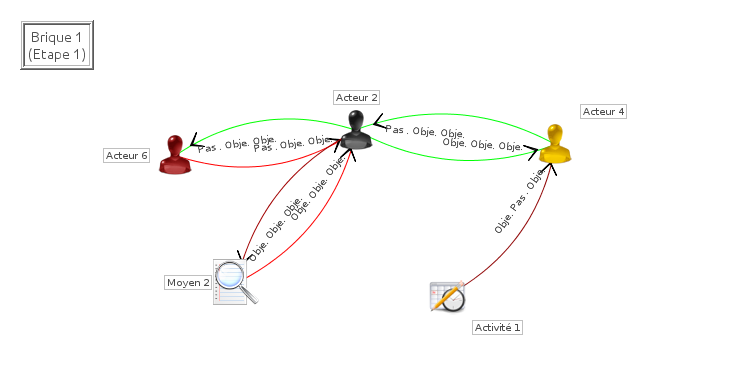
\includegraphics[width=12cm]{images/exportOrigin.png}
}
\caption{A brick during the relation edition.}
\vspace*{15pt}
\Ovalbox{
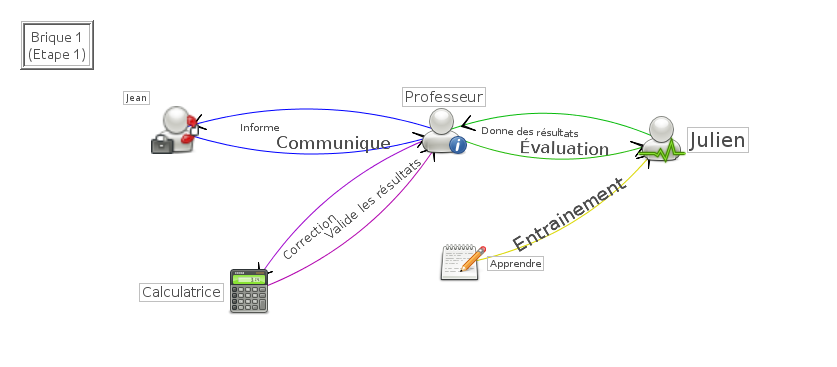
\includegraphics[width=12cm]{images/exportModifie.png}
}
\caption{The same after the export preparation}
\label{personalisation}
\end{figure}
